\chapter{My first chapter}
\begin{center}
{A. Student$^{1}$, B. Supervisor$^{2,3}$}\\
\end{center}
\textit{Author Affiliations:}\\
\normalsize{$^{1}$Department of Biology, McGill University}\\
\normalsize{$^{2}$Scientific Services, Canadian Government}\\
\normalsize{$^{3}$Department of Paranormal Sciences, Faculty of Pseudoscience, University of Transubstantiation}\\
\section{Abstract}
\lipsum[66]
\\
\section{Introduction}
\lipsum[66]\\
\section{Methods}

\subsection*{Study Site}
\lipsum[66]\\
\subsection*{Sampling}
\lipsum[66]\\
\subsection*{Analyses}
\lipsum[66]\\
\section{Results}
\lipsum[66](Fig. \ref{fig:S_XS_composition}).
\\
\section{Discussion}
\lipsum[66]
\\

\newpage
\section*{Figures \& Tables}

\begin{figure}[!ht]
  \centering
    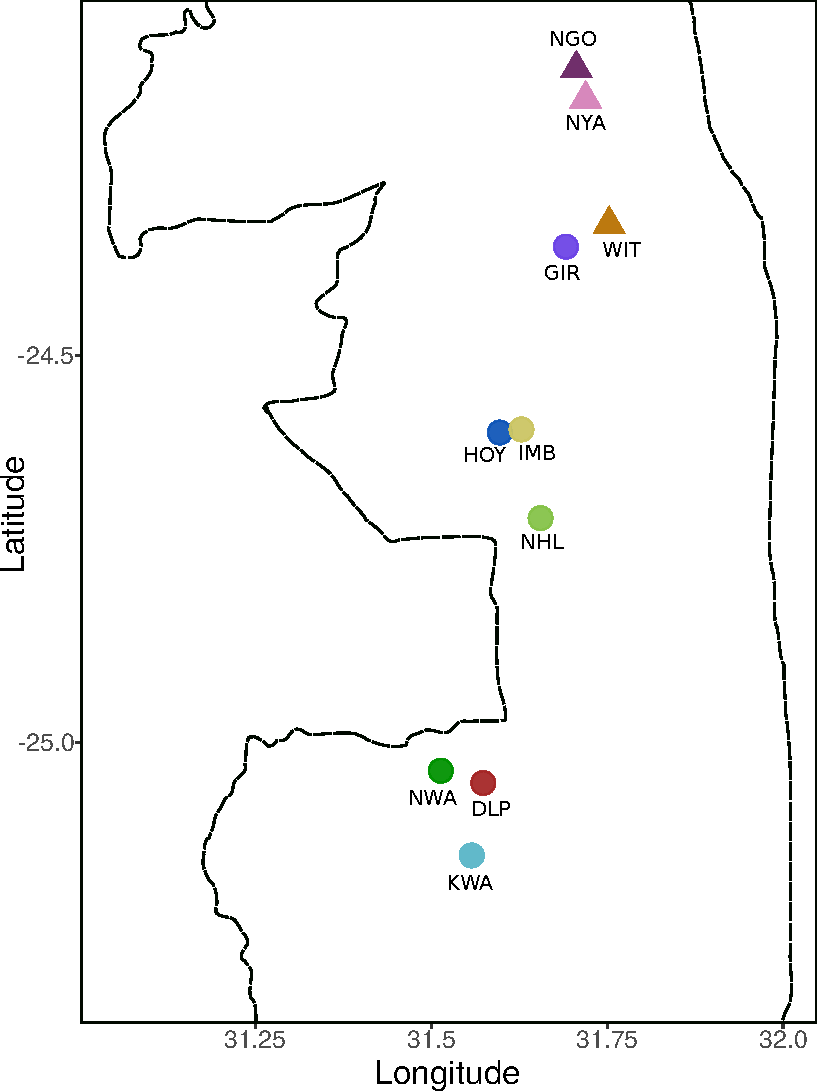
\includegraphics[width=0.5\textwidth]{plots_tables/chap_1/kruger_points_simple.pdf}
  \caption{Map of site locations with park boundary indicated by dashed line. Circles represent sites filled by boreholes while triangles represent sites filled by river water via pipeline troughs.}
  \label{fig:map}
\end{figure}

\begin{table}[h!]
\centering
\begin{tabular}{llllll|l}
  \hline
  \hline
  Site & Weeks & S & XS & Daily & A/B & Total\\
  \hline
  Nhlanguleni (NHL) 	& 3 & 0 & 0 & 0 & Yes & 6 \\ 
  Nwaswitshaka (NWA) 	& 3 & 1 & 1 & 4 & Yes & 18 \\ 
  De LaPorte (DLP) 		& 1 & 1 & 1 & 0 & Yes & 6 \\ 
  Kwaggas Pan (KWA) 	& 2 & 1 & 1 & 0 & Yes & 8\\ 
  Girivana (GIR) 		& 3 & 0 & 0 & 0 & Yes & 6 \\ 
  Witpens (WIT) 		& 3 & 0 & 0 & 0 & Yes & 6 \\ 
  Imbali (IMB) 			& 3 & 0 & 0 & 0 & Yes & 6 \\ 
  Hoyo Hoyo (HOY) 		& 3 & 1 & 1 & 0 & Yes & 10 \\ 
  Nyamarhi (NYA) 		& 3 & 1 & 1 & 0 & Yes & 10 \\ 
  Ngosto North (NGO) 	& 3 & 1 & 1 & 0 & Yes &10 \\ 
  BLANK 				& 2 & 0 & 0 & 0 & No & 2 \\ 
  \hline
   						& 29 & 6 & 6 & 4 & & 88 \\
  \hline
  \hline
\end{tabular}
\caption{Samples sequences, broken down by number of weekly samples, number of site-times for which S (50 mL) and XS (15 mL) samples were filtered, additional daily samples taken, whether A/B samples were taken, and the resulting total number of samples sequenced per site.}
\label{tab:samples}
\end{table}
